\documentclass[11pt]{article}

\usepackage[margin=1in]{geometry}
\usepackage{graphicx}
\usepackage{amsmath}
\usepackage{booktabs}
\usepackage{caption}
\usepackage{subcaption}
\usepackage{xcolor}
\usepackage[colorlinks=true,linkcolor=blue,citecolor=blue,urlcolor=blue]{hyperref}

% Figures are bundled in this directory (presentation/paper/figs/) so the paper
% dir is self-contained; refresh them from presentation/figs/ with `make figs`.
\graphicspath{{figs/}}
% numbers.tex — canonical quantities, cited once so prose never disagrees.
% Canonical window config: half_window = 500 bp (1 kb window), buffer = 0.
% Counts at this config come from presentation/window_sweep.csv (row length=1000).
%
% NOTE: pipeline_summary.md quotes 26,267 windows for the legacy demo config
% (buffer = 50). This document standardizes on buffer = 0.

% Windowing (half_window = 500, buffer = 0)
\newcommand{\nWindows}{23{,}138}            % total windows over the VCF
\newcommand{\variantsPerWindow}{2.31}       % mean distinct haplotypes per window
\newcommand{\meanTokens}{168}               % mean Carbon 6-mer tokens / 1 kb window

% Forward-call accounting: naive vs. variant cache
\newcommand{\naiveForwards}{8{,}861{,}854}   % naive sample x window full forwards
\newcommand{\cacheRefForwards}{23{,}138}     % full reference forwards under the cache
\newcommand{\cacheFactor}{383$\times$}       % naive -> variant-cache reduction

% Embedding fidelity (fig 04 / vc_degradation.csv; Carbon-500M, fp32)
\newcommand{\varCosMean}{0.99996}            % mean per-SNP-token cosine vs true alt
\newcommand{\poolCosMean}{0.99999}           % mean window-pooled cosine vs true alt
\newcommand{\relerrOneSnp}{2.5\times10^{-3}} % pooled rel. L2 error at 1 SNP
\newcommand{\relerrEightSnp}{8.4\times10^{-3}} % pooled rel. L2 error at ~8 SNPs

% Autoregressive SNP fine-tune (fig 05; Carbon-500M via the cache, 90% train)
\newcommand{\arNllStart}{5.94}
\newcommand{\arNllEnd}{5.03}
\newcommand{\arPplStart}{382}
\newcommand{\arPplEnd}{153}


\title{The Variant Cache: Efficient Genome--Language--Model Inference and
Training over a Cohort of Near-Reference Haplotypes}
\author{Andrew Dickson}
\date{\today}

\begin{document}
\maketitle

\begin{abstract}
A cohort of resequenced genomes differs from the reference assembly only at a
sparse set of SNPs. Embedding or scoring every (sample, window) pair with a DNA
language model therefore repeats almost identical computation millions of times.
We introduce the \emph{variant cache}: a forward pass that runs the reference
window once, caches its per-layer residual stream, and recomputes only the
handful of variant tokens, which attend back into the cached reference context
via a log-sum-exp merge of two attentions. The result is mathematically a single
softmax over the union of reference and variant keys, so the cache is exact for
an isolated SNP and degrades gracefully as SNPs co-occur. Against the naive pass
that runs every sample's window through the full model, it cuts full
language-model forwards over the rice \textit{Oryza sativa} panel by
\cacheFactor{}. We validate the method along two
axes: (A) cache embeddings are near-identical to the true full-forward
embeddings (mean per-SNP-token cosine \varCosMean{}) and the cache supports
efficient autoregressive fine-tuning on the SNP-prediction objective; and (B)
window embeddings produced through the cache yield the same downstream
trait-prediction results and the same population structure as
embeddings produced by the standard forward pass.
\end{abstract}

\section{Introduction}
\label{sec:intro}
We work with the rice diversity panel: a biallelic SNP VCF
(\texttt{sativas413\_msu7\_final.vcf}) over an inbred \textit{O.\ sativa} cohort,
plus the IRGSP-1.0 reference FASTA. The genomes are tiled into fixed-length
windows; each window is embedded (or scored) by a pretrained DNA language model
--- DNABERT-2~\cite{zhou2023dnabert2} (bidirectional, ALiBi~\cite{press2022alibi})
or Carbon~\cite{carbon2024} (decoder-only, RoPE~\cite{su2021rope}). Genomic
language models of this kind~\cite{zhou2023dnabert2,dallatorre2023nucleotide}
learn representations transferable to downstream tasks such as trait prediction
over the rice diversity panel~\cite{zhao2011rice}. Because the
samples are near-reference, the work is dominated by redundancy: at a 1\,kb
window over this panel a naive pass would run \naiveForwards{} full forwards
(samples $\times$ windows), almost all of them re-embedding sequence that is
byte-for-byte the reference. This document describes the variant cache that
removes that redundancy (Section~\ref{sec:method}) and the experiments that
establish it is both faithful and benign (Section~\ref{sec:experiments}).
All quantities use the canonical window config: half-window $500$\,bp (a
$1$\,kb window), buffer $0$.

\section{The Variant Cache Model}
\label{sec:method}

\subsection{Setup: the naive cost over a near-reference cohort}
A SNP-window partitioner greedily tiles each chromosome into fixed-length windows
so every SNP sits at least \texttt{buffer} bp inside a window (\nWindows{}
windows at the canonical config). Each sample's window differs from the reference
only at its alt alleles. The \emph{naive} approach embeds (or scores) every
sample's every window with a full model forward, spending \naiveForwards{}
forwards (samples $\times$ windows) --- almost all of them re-embedding sequence
that is byte-for-byte the reference. The variant cache removes exactly this
redundancy: it computes the reference window once and reuses it across every
sample, recomputing only the few tokens that actually carry a variant.

\subsection{The cache forward pass}
After tokenization a window's token sequence is nearly identical across samples:
only the 6-mer tokens whose span contains an alt allele differ
(Figure~\ref{fig:decomp}). The variant cache exploits this. Given one reference
window we want the hidden states of a few \emph{variant} tokens substituted at
chosen positions, without re-running the whole model per variant:
\begin{enumerate}
  \item \textbf{Reference pass.} Run the reference once and cache the
  \emph{per-layer residual-stream input} entering every layer (the K/V source
  the variant update attends to).
  \item \textbf{Variant recompute.} At each layer, recompute only the variant
  tokens. A variant query at original position $p$ attends to
  $\{\text{reference keys at non-variant positions}\} \cup \{\text{variant keys}\}$,
  which is exactly a single softmax over the union of those two key sets. We
  never materialize the reference at the variant batch size; instead we run two
  attentions~\cite{vaswani2017attention} --- variant$\to$reference and
  variant$\to$variant --- and merge them with the log-sum-exp identity, the same
  streaming-softmax combine used by online-softmax and FlashAttention
  formulations~\cite{milakov2018online,dao2022flashattention}
  \[
    \mathrm{lse} = \log\!\big(e^{\mathrm{lse}_c} + e^{\mathrm{lse}_s}\big),\qquad
    \mathrm{attn} = e^{\mathrm{lse}_c-\mathrm{lse}}\,\mathrm{out}_c
                  + e^{\mathrm{lse}_s-\mathrm{lse}}\,\mathrm{out}_s .
  \]
\end{enumerate}
Position information enters per backbone: Carbon rotates Q/K by absolute position
(RoPE~\cite{su2021rope}) and is causal, so the union of reference and variant
keys $\le p$ is a clean partition; DNABERT-2 adds an ALiBi
bias~\cite{press2022alibi} and is bidirectional, so the cross-attention mask
drops the variant positions to avoid double counting. Carbon's backbone is a
Llama-style stack~\cite{touvron2023llama} with grouped-query
attention~\cite{ainslie2023gqa}, whose grouped K/V heads are expanded before the
merge.
Figure~\ref{fig:forward} contrasts the two passes: standard work scales as
$B\cdot T\cdot L$ (batch $\times$ tokens $\times$ layers); the cache scales as
$(T + B\cdot V)\cdot L$ with the number of variant tokens $V \ll T$.

\begin{figure}[t]
  \centering
  \begin{subfigure}{0.40\textwidth}
    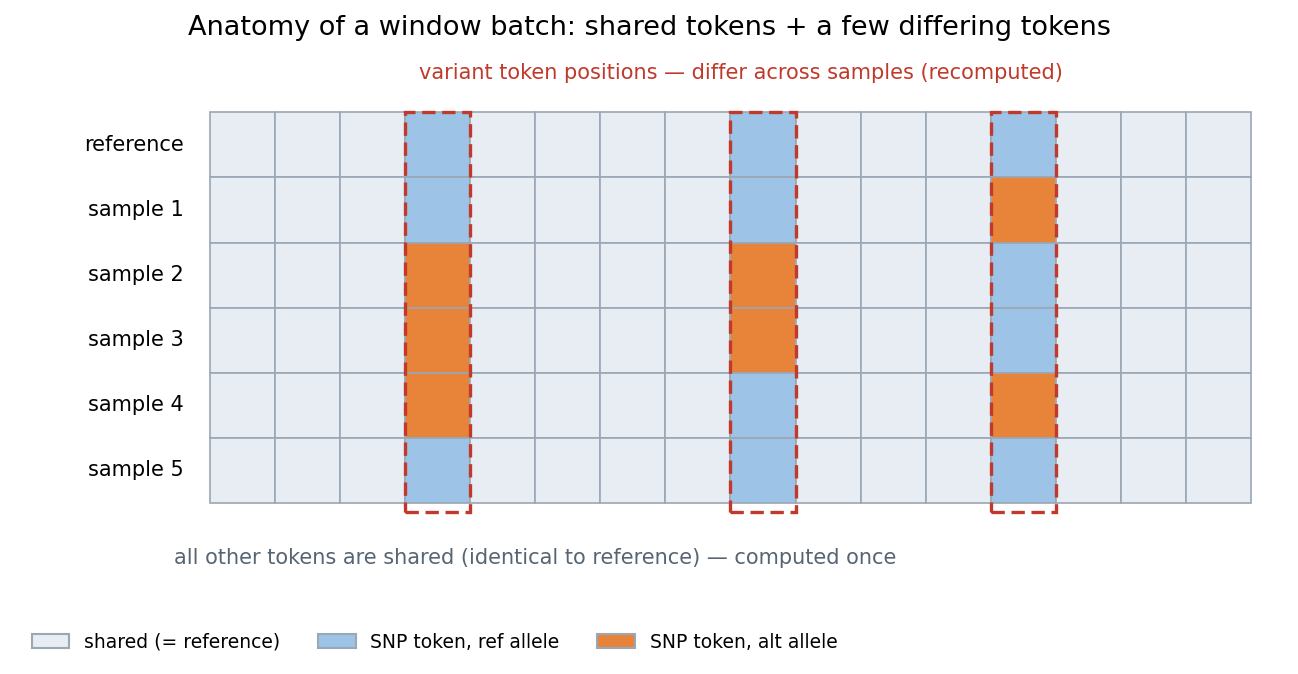
\includegraphics[width=\linewidth]{06_vc_batch_decomposition.png}
    \caption{Batch anatomy: shared (grey) vs.\ the few differing SNP columns.}
    \label{fig:decomp}
  \end{subfigure}\hfill
  \begin{subfigure}{0.56\textwidth}
    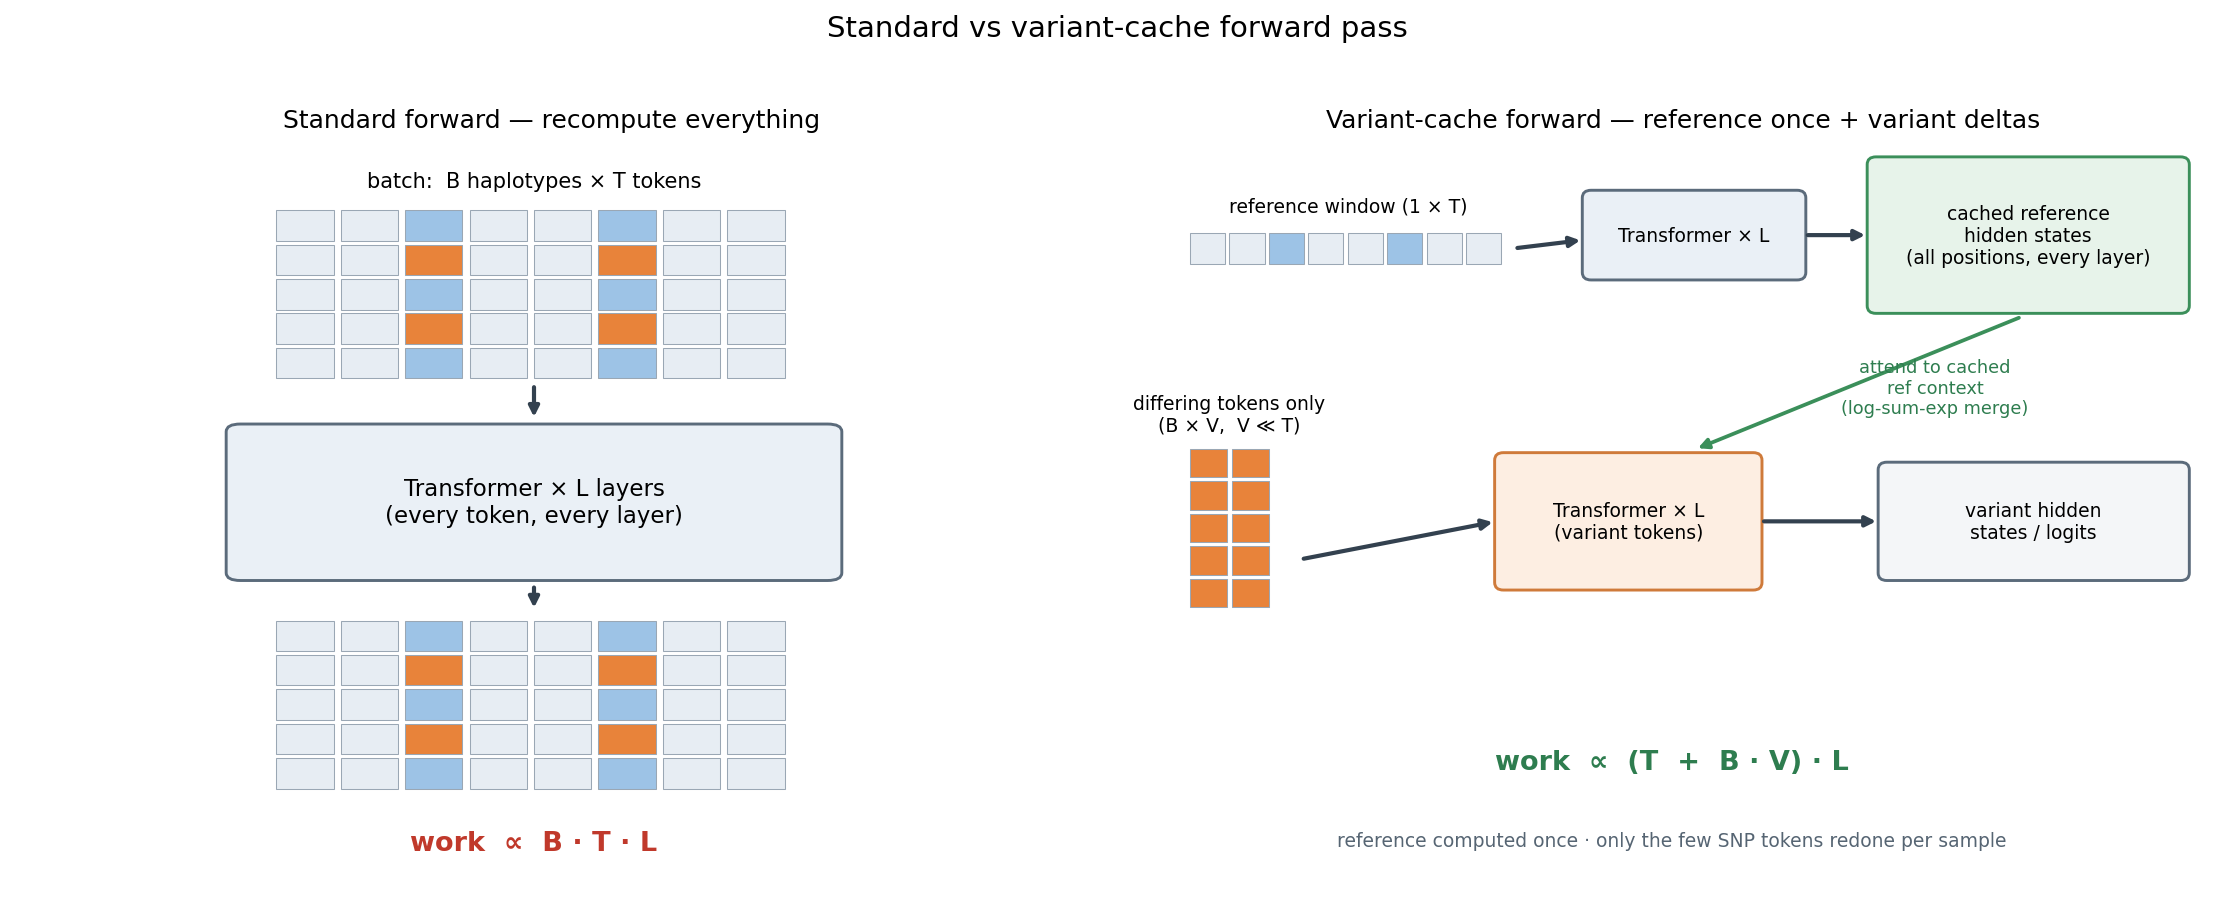
\includegraphics[width=\linewidth]{07_vc_forward_comparison.png}
    \caption{Standard forward ($B\cdot T\cdot L$) vs.\ the variant cache
    ($(T+B\cdot V)\cdot L$): reference cached once, variant tokens recomputed and
    merged via log-sum-exp.}
    \label{fig:forward}
  \end{subfigure}
  \caption{The variant-cache forward pass.}
  \label{fig:method}
\end{figure}

\subsection{Forward-call accounting and correctness}
Against the naive \naiveForwards{} full forwards, the variant cache runs one full
reference forward per window --- \cacheRefForwards{} in total --- plus cheap
partial recomputes of only the variant tokens, a \cacheFactor{} reduction in full
language-model forwards. Each backbone ships two implementations: an
\texttt{efficient} backend (the log-sum-exp merge) and a \texttt{bruteforce}
oracle that runs full-sequence layers and clamps the non-variant positions back
to the frozen reference after each layer. The oracle materializes exactly the
activations the cache avoids, so \texttt{efficient} must equal \texttt{bruteforce}
up to fp32 numerics; an \emph{identity probe} (substituting the reference's own
tokens) further requires the cache to reproduce the ordinary forward exactly.
Table~\ref{tab:correctness} reports these checks
(\texttt{model\_dev/test\_carbon\_variant\_cache.py}).

% Generated by presentation/make_correctness_table.py (needs the 500M checkpoint).
% A placeholder ships in the repo so the document builds before the GPU run.
% Placeholder — regenerate with presentation/make_correctness_table.py (needs the
% Carbon-500M checkpoint). Values below are the expected/representative outcomes
% of model_dev/test_carbon_variant_cache.py and are overwritten by that script.
\begin{table}[t]
  \centering
  \caption{Variant-cache correctness checks on Carbon-500M (fp32). The efficient
  log-sum-exp merge matches the brute-force oracle to numerical precision, and
  the identity probe reproduces the ordinary forward; real substitutions are an
  approximation, reported (not asserted). \emph{Placeholder values --- rerun
  \texttt{make\_correctness\_table.py}.}}
  \label{tab:correctness}
  \begin{tabular}{lcc}
    \toprule
    Check & max abs.\ diff & cosine \\
    \midrule
    Efficient vs.\ brute-force        & $<10^{-3}$ & $1.0000$ \\
    Identity probe vs.\ full forward  & $<10^{-3}$ & $1.0000$ \\
    Real substitutions (approx.)      & ---        & $\sim 0.99$ \\
    \bottomrule
  \end{tabular}
\end{table}


\section{Experiments}
\label{sec:experiments}

\subsection{Window-length design tradeoff}
\label{sec:exp-window}
\textbf{What I did.} The window length sets the two quantities that drive the
cache's cost: the tokens per window $T$ and the number of distinct haplotypes per
window (the $B$ in the $B\cdot V$ recompute term). Sweeping $L$ from $2$\,bp to
$1$\,Mb I measured the mean Carbon 6-mer tokens per window, the mean distinct
haplotypes per window, and the number of distinct window sequences
(\texttt{presentation/count\_windows.py} $\to$ \texttt{window\_sweep.csv} $\to$
\texttt{plot\_window\_sweep.py}). No model forward is needed.
\textbf{Result} (Figure~\ref{fig:window_sweep}). Tokens/window grow linearly
($\sim L/6$) and distinct haplotypes/window rise from $2$ to $135$. Short windows
stay near-reference --- few variant tokens, cheap and accurate to cache --- while
long windows pack more co-segregating SNPs, so both $T$ and $B$ explode. The
$1$\,kb canonical window sits in the cheap regime (\meanTokens{} tokens,
\variantsPerWindow{} haplotypes/window).

\begin{figure}[t]
  \centering
  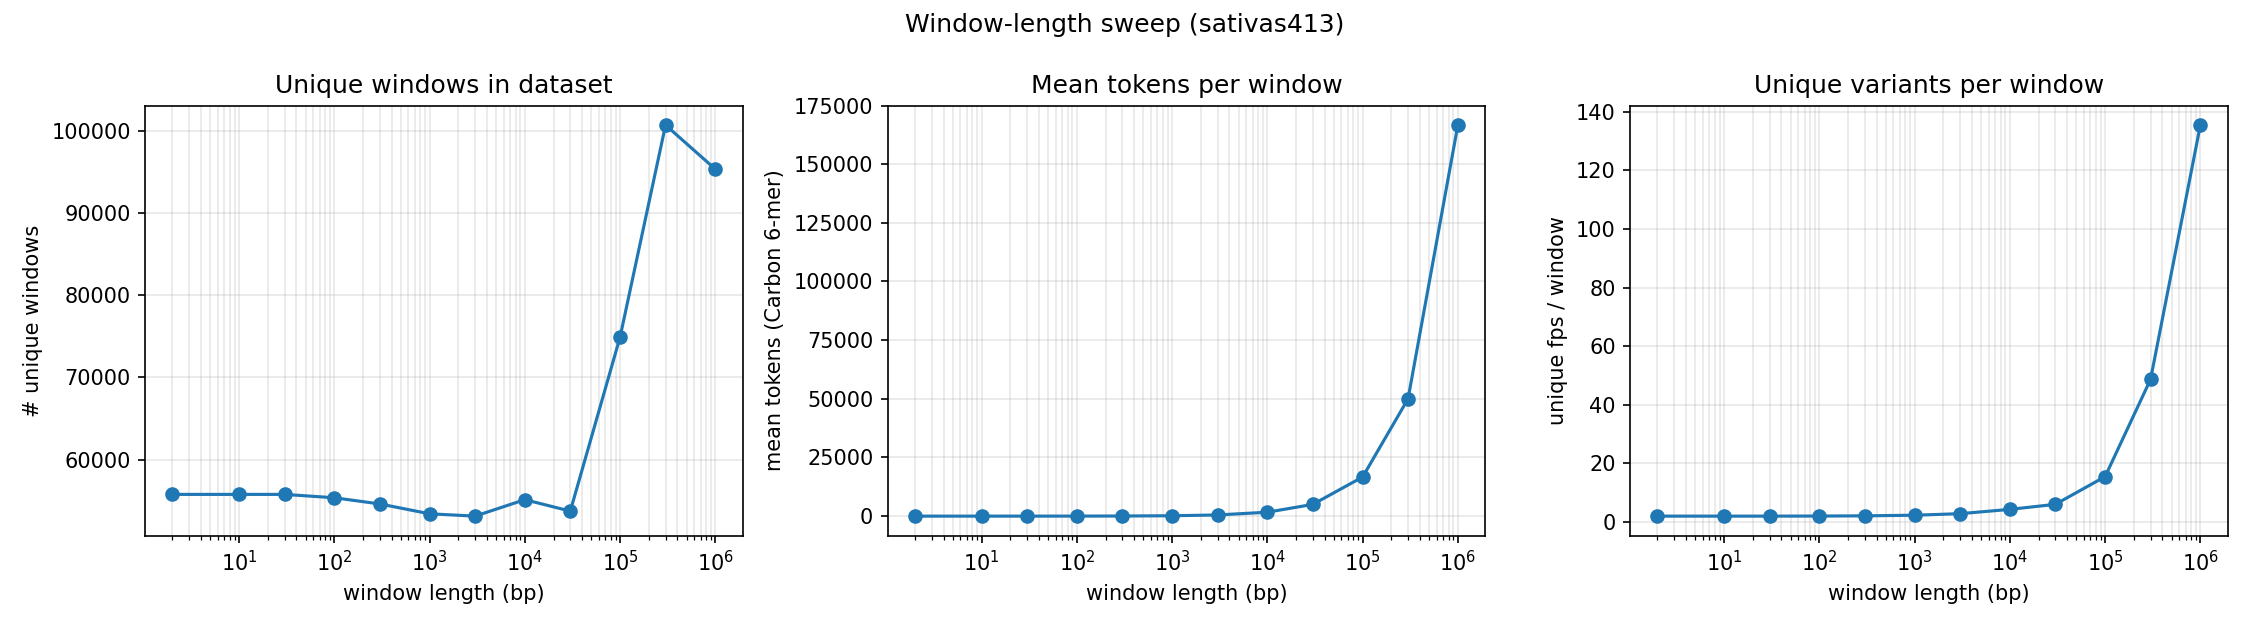
\includegraphics[width=0.95\linewidth]{01_window_sweep.png}
  \caption{Distinct window sequences, mean tokens/window, and haplotypes/window
  vs.\ window length (log $x$).}
  \label{fig:window_sweep}
\end{figure}

\subsection{Embedding fidelity vs.\ number of concurrent SNPs (Claim A)}
\label{sec:exp-fidelity}
\textbf{What I did.} For thousands of variant windows I compared three
embeddings of the alt haplotype: \emph{true} (full Carbon-500M forward of the alt
sequence), \emph{cache} (frozen reference + recomputed SNP tokens), and
\emph{ref} (reference-only baseline). I report per-SNP-token cosine to the true
forward and the window-pooled relative $L^2$ error, binned by the number of SNP
tokens in the window
(\texttt{model\_dev/compare\_variant\_cache\_embeddings.py} $\to$
\texttt{vc\_degradation.csv} $\to$ \texttt{plot\_vc\_degradation.py}).
\textbf{Result} (Figure~\ref{fig:degradation}). Per-SNP-token cosine is
$\approx 1.0$ at a single SNP and only drifts to $\sim 0.999$ by 9 concurrent
SNPs (mean \varCosMean{}); pooled relative error rises from $\relerrOneSnp$ at
1 SNP to $\relerrEightSnp$ at $\sim 8$ SNPs. The cache is near-exact for isolated
SNPs and degrades gracefully as SNPs co-occur --- exactly the frozen-reference
approximation's expected behavior.

\begin{figure}[t]
  \centering
  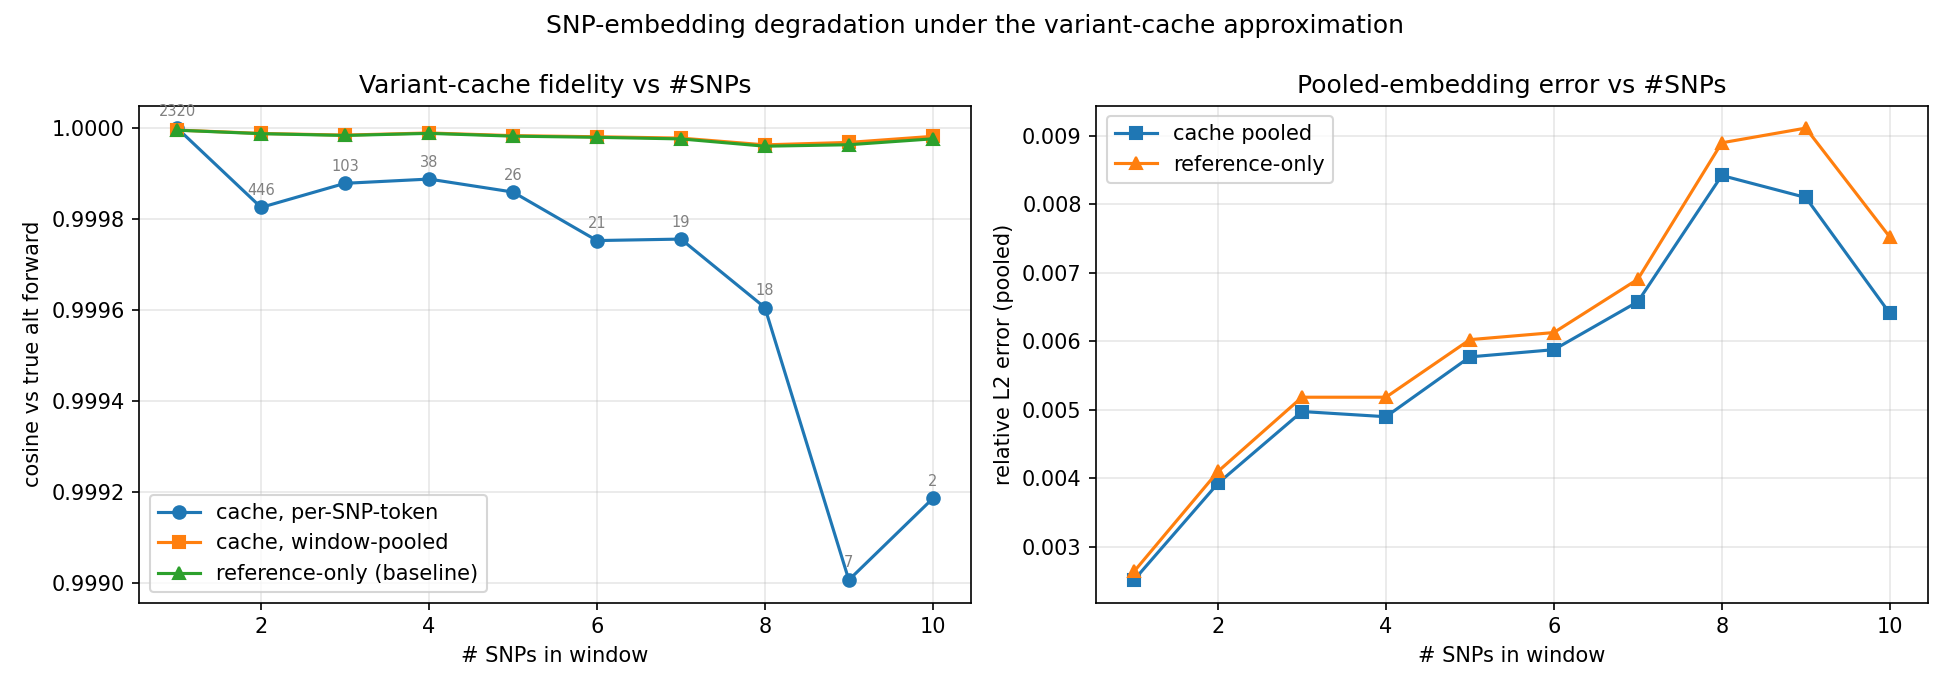
\includegraphics[width=0.95\linewidth]{04_vc_degradation.png}
  \caption{Cache fidelity vs.\ \#SNPs. Left: cosine to the true alt forward
  (per-SNP-token and window-pooled, with the reference-only baseline). Right:
  pooled-embedding relative $L^2$ error.}
  \label{fig:degradation}
\end{figure}

\subsection{Autoregressive SNP prediction through the cache (Claim A)}
\label{sec:exp-ar}
\textbf{What I did.} I fine-tuned Carbon-500M on the next-token negative
log-likelihood of the SNP-bearing 6-mer tokens, \emph{through the variant cache}
(\texttt{variant\_ar/train.py --backend cache}), on the 90\% training split of
the variant windows ($\texttt{--val-frac}\ 0.1$). The cache loss is the exact
objective's frozen-reference approximation, and \texttt{--backend exact}
optimizes the identical loss on the stock model for a directly comparable
baseline.
\textbf{Result} (Figure~\ref{fig:ar}). Validation improves every epoch ---
log-likelihood on SNP tokens rises (NLL $\arNllStart \to \arNllEnd$) and
perplexity falls $\arPplStart \to \arPplEnd$ --- while noisy train
log-likelihood climbs higher, the gap reflecting mild overfitting on the bounded
demo subset. The cache supports end-to-end fwd+bwd fine-tuning, not just
inference.

\begin{figure}[t]
  \centering
  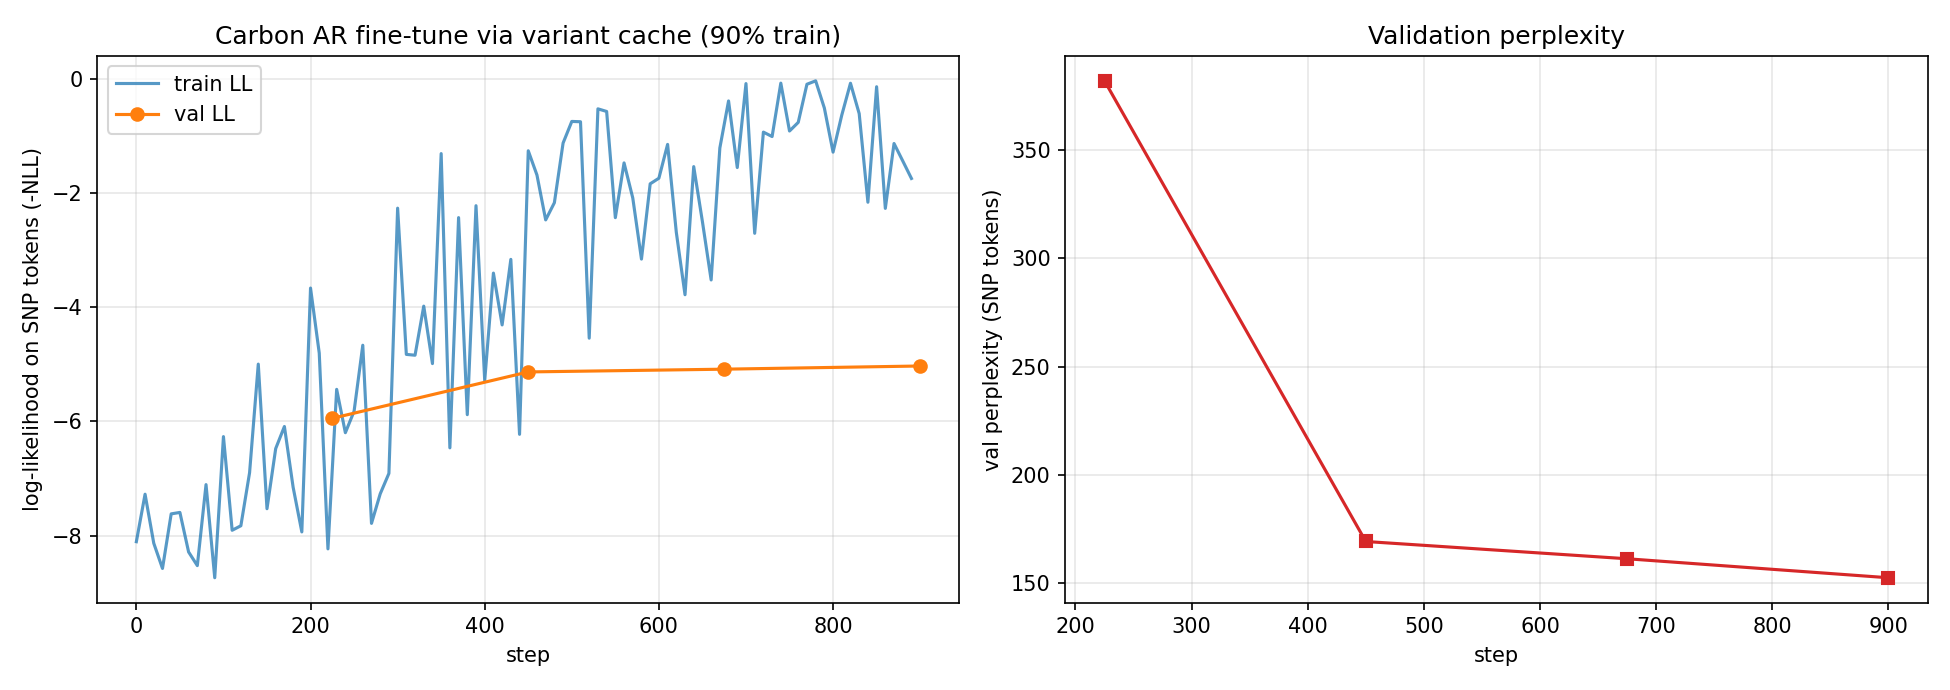
\includegraphics[width=0.95\linewidth]{05_ar_curves.png}
  \caption{Carbon AR fine-tune via the variant cache (90\% train). Left:
  train/val log-likelihood on SNP tokens. Right: validation perplexity.}
  \label{fig:ar}
\end{figure}

\subsection{Downstream trait prediction is unchanged (Claim B)}
\label{sec:exp-head}
\textbf{What I did.} On precomputed window-embedding caches I trained
trait-prediction heads, sweeping the window-aggregation diff
(\emph{absolute} / \emph{centered} / \emph{refdelta}), head type, pooling, and
the embedding cache itself (variant-cache vs.\ full-forward), logging train/val
MSE and Pearson correlation per step (\texttt{train\_pipeline/train\_head.py},
\texttt{run\_head\_sweep.sh}; plotted in \texttt{render\_all.ipynb}).
\textbf{Result} (Figure~\ref{fig:head}). The aggregation diffs separate cleanly
in both the mean curves and per-trait correlation, and heads trained on
variant-cache embeddings track those trained on full-forward embeddings ---
downstream predictive quality is preserved.

\begin{figure}[t]
  \centering
  \begin{subfigure}{0.49\textwidth}
    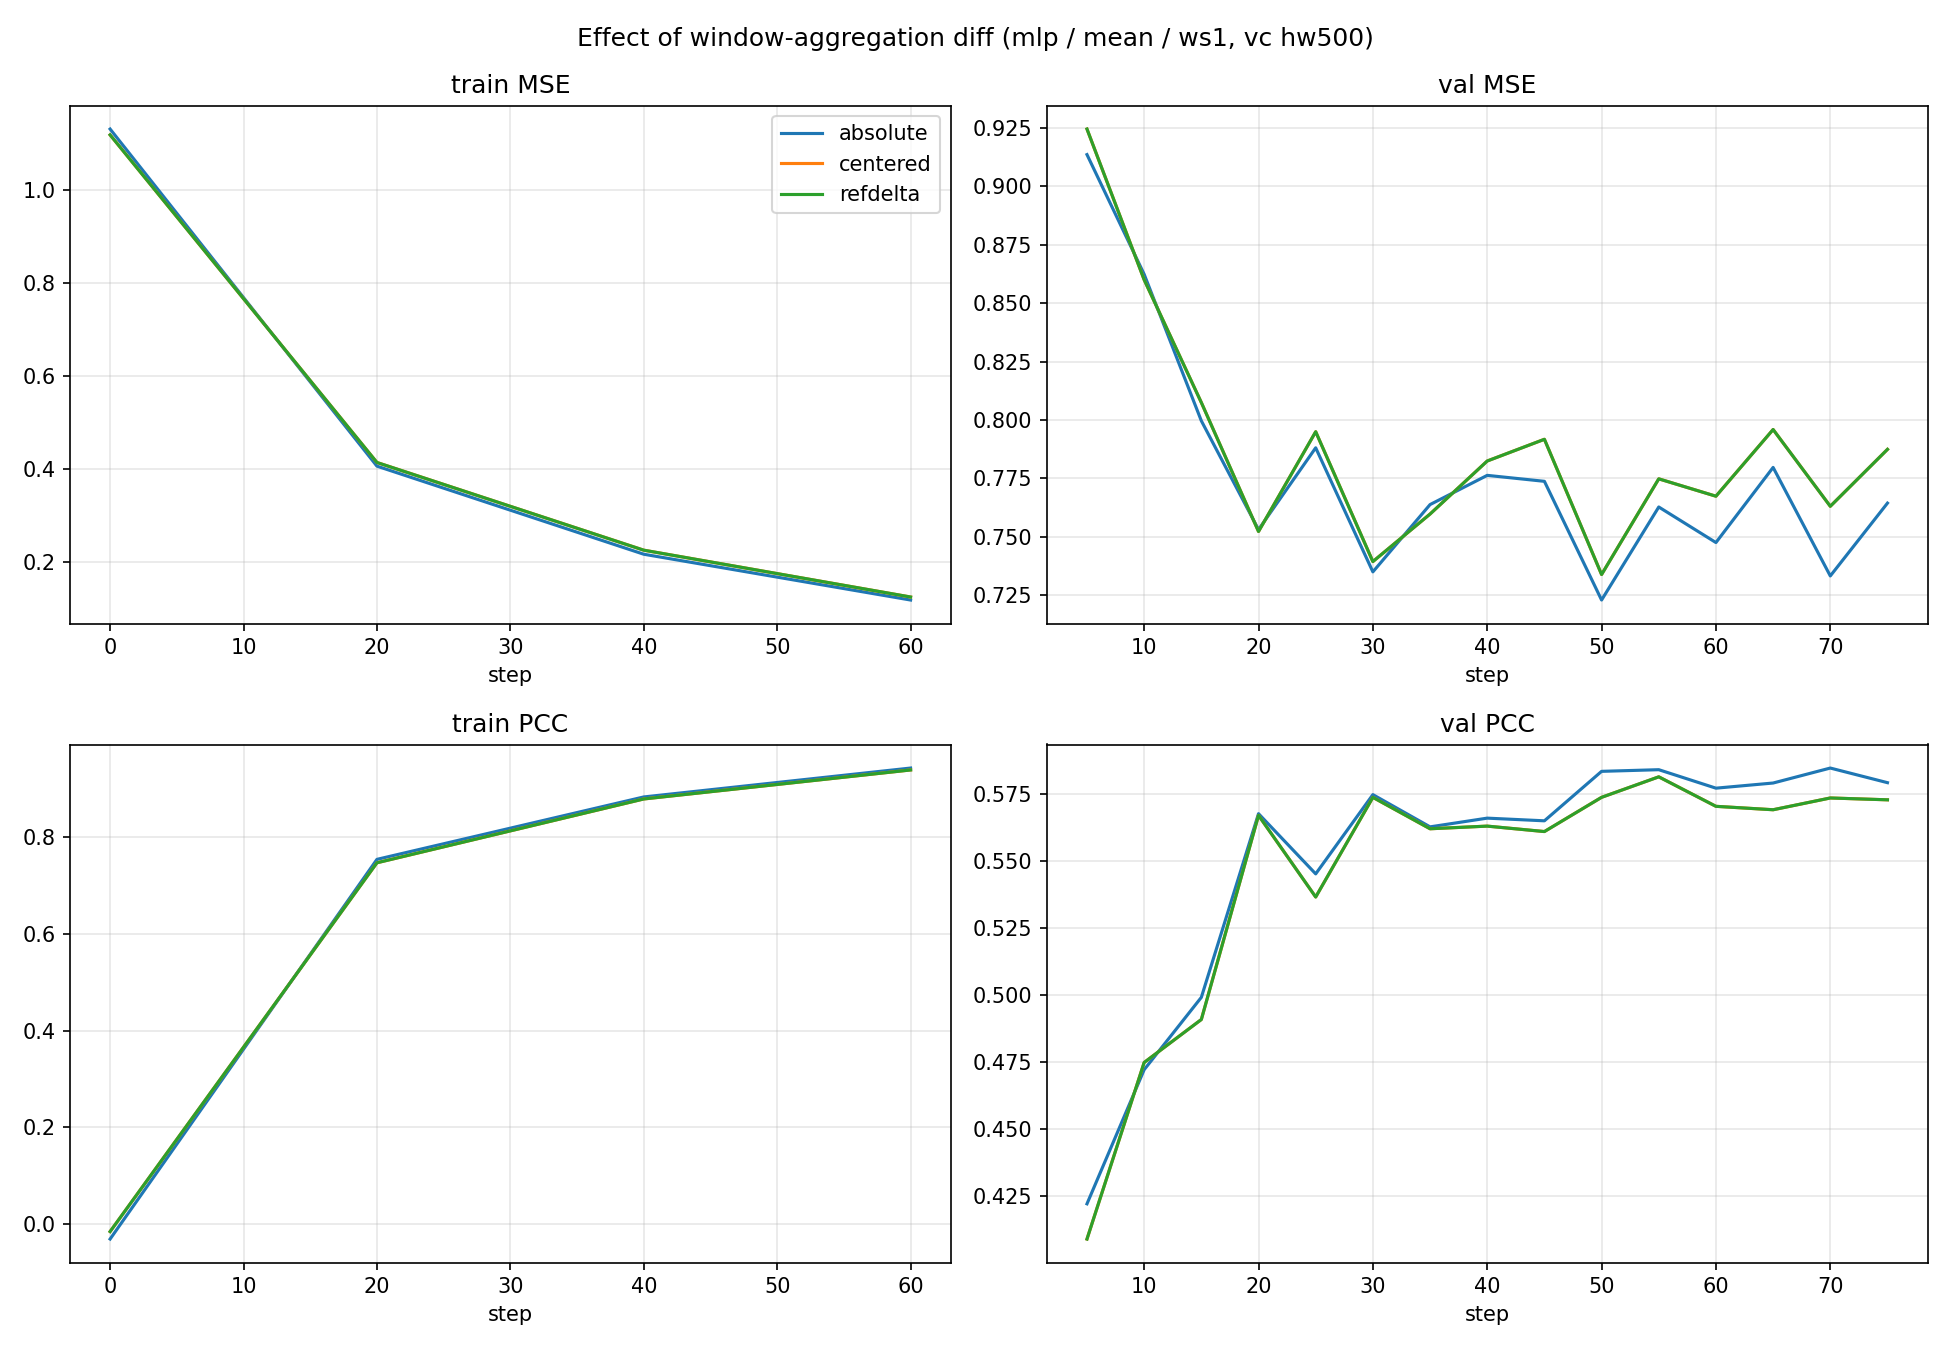
\includegraphics[width=\linewidth]{02_diff_curves.png}
    \caption{Train/val MSE and PCC over training, per aggregation diff.}
    \label{fig:diff_curves}
  \end{subfigure}\hfill
  \begin{subfigure}{0.49\textwidth}
    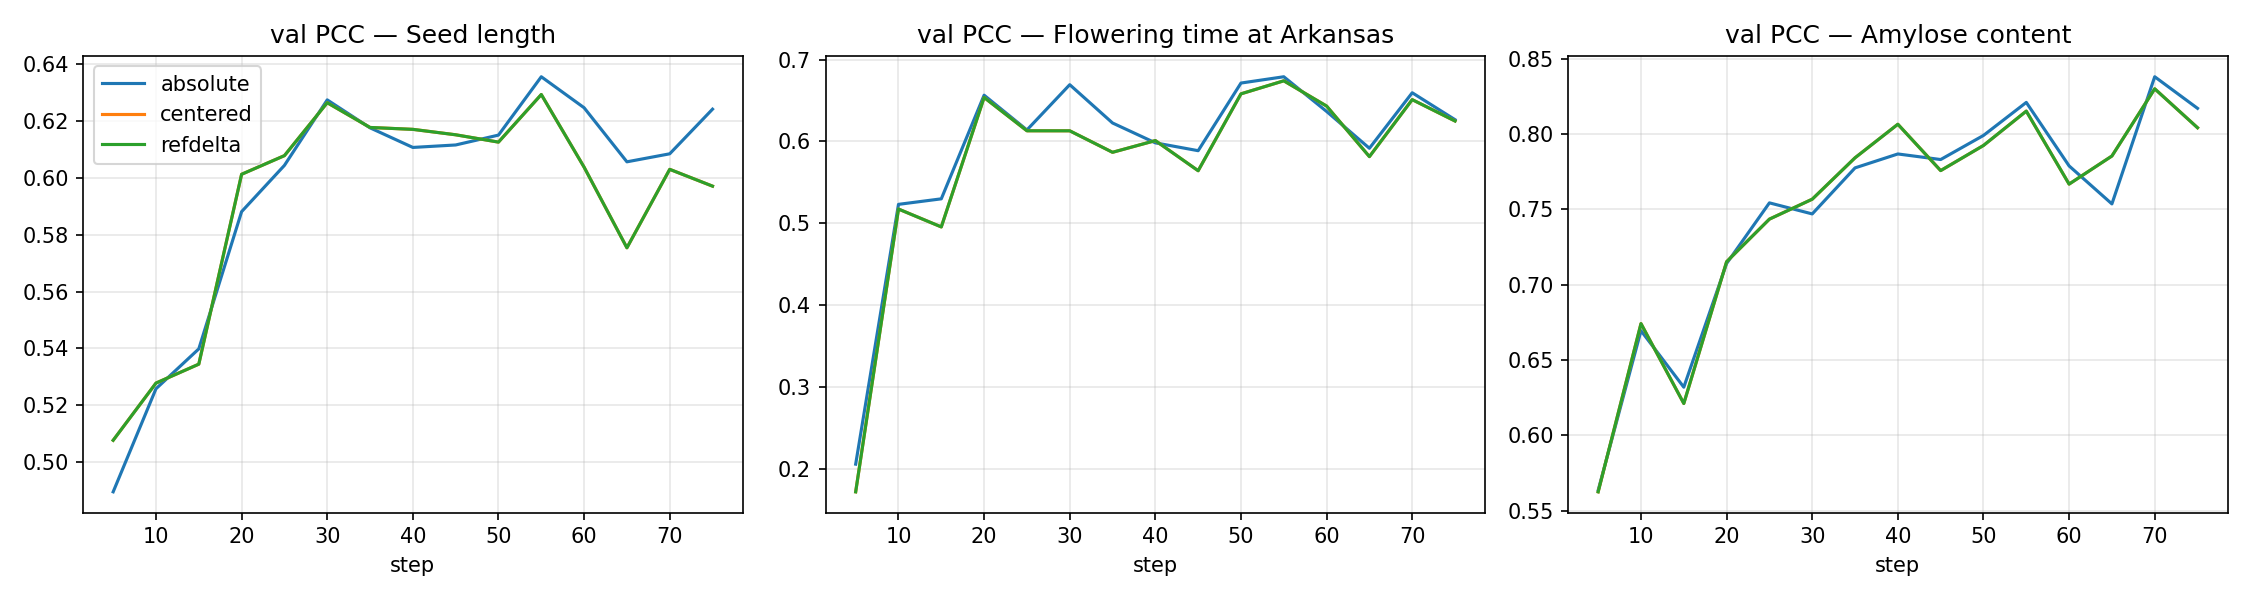
\includegraphics[width=\linewidth]{02_per_trait_pcc.png}
    \caption{Validation PCC per trait.}
    \label{fig:per_trait}
  \end{subfigure}
  \caption{Head-training curves across aggregation diffs.}
  \label{fig:head}
\end{figure}

\subsection{Downstream representation structure is unchanged (Claim B)}
\label{sec:exp-umap}
\textbf{What I did.} I projected the per-sample embeddings to 2-D with UMAP~\cite{mcinnes2018umap}
under each preprocessing recipe (all vs.\ SNP-only windows; Carbon vs.\
DNABERT-2; sum+standardize vs.\ center+LayerNorm+mean), coloring by inferred
subpopulation (SNP PC1 quartile) (\texttt{presentation/umap\_preprocessing.py}).
\textbf{Result} (Figure~\ref{fig:umap}). Every recipe recovers subpopulation
structure, and the variant-cache panels mirror their full-forward counterparts:
the cache preserves the embedding geometry the downstream models rely on.

\begin{figure}[t]
  \centering
  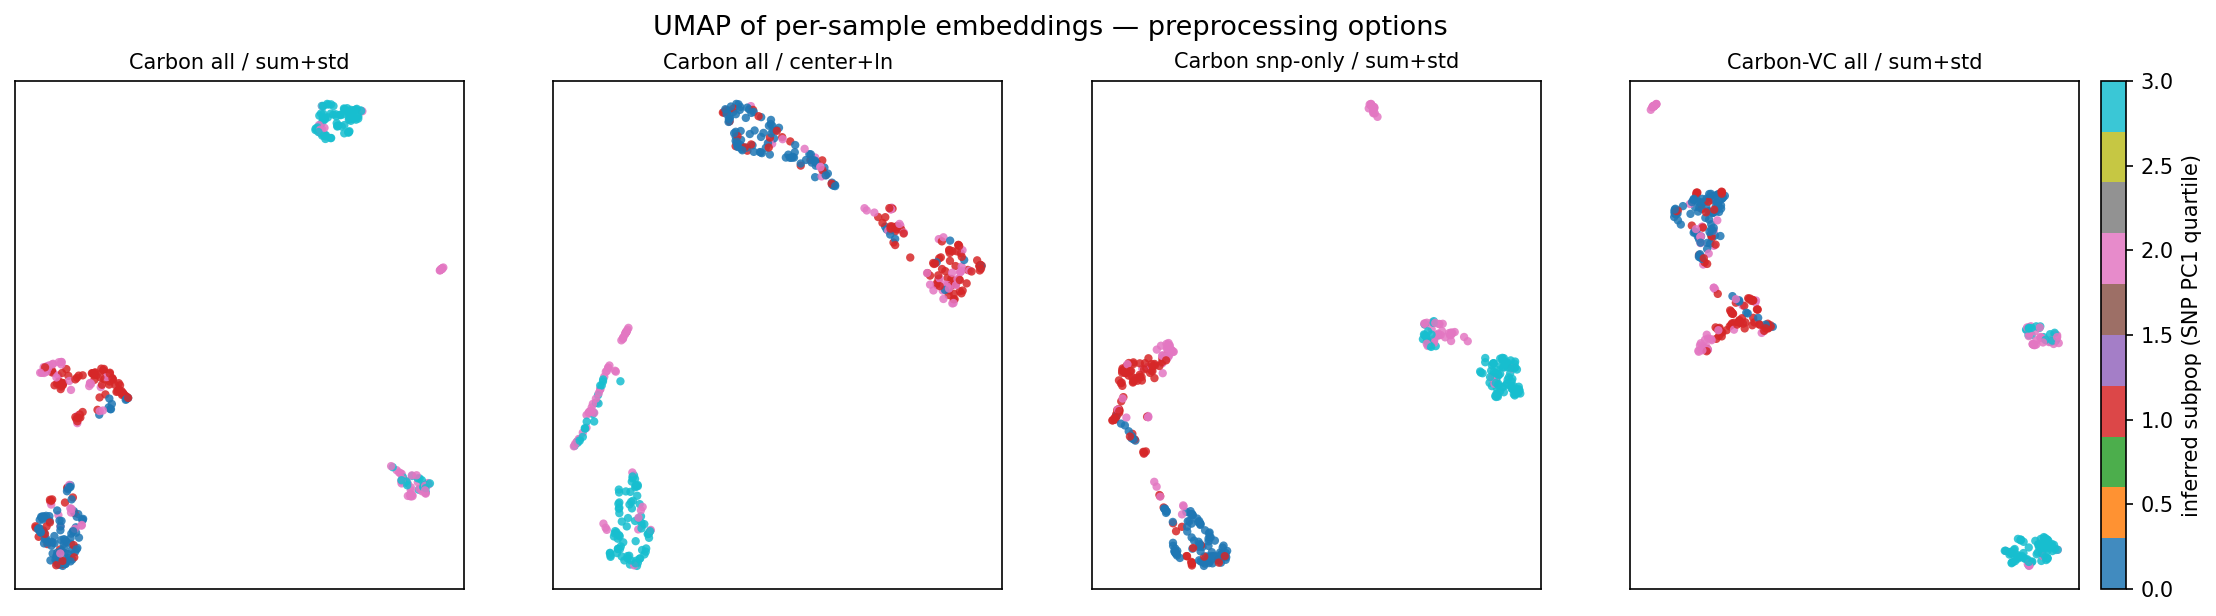
\includegraphics[width=0.95\linewidth]{03_umap_grid.png}
  \caption{UMAP of per-sample embeddings across preprocessing options, colored
  by inferred subpopulation. Variant-cache panels mirror full-forward.}
  \label{fig:umap}
\end{figure}

\subsection{Cache vs.\ full-forward window embeddings, directly (Claim B)}
\label{sec:exp-bitwise}
\textbf{What I did.} I aligned the variant-cache window-embedding table to the
full-forward table window-by-window and measured the per-window $L^2$ difference
(\texttt{train\_pipeline/compare\_embeddings.py --csv-out} $\to$
\texttt{presentation/plot\_cache\_vs\_fullforward.py}).
\textbf{Result} (Figure~\ref{fig:bitwise}). The per-window difference is a tiny
fraction of the embedding norm, so the two caches are interchangeable as
downstream inputs --- the most direct statement of Claim B.

\begin{figure}[t]
  \centering
  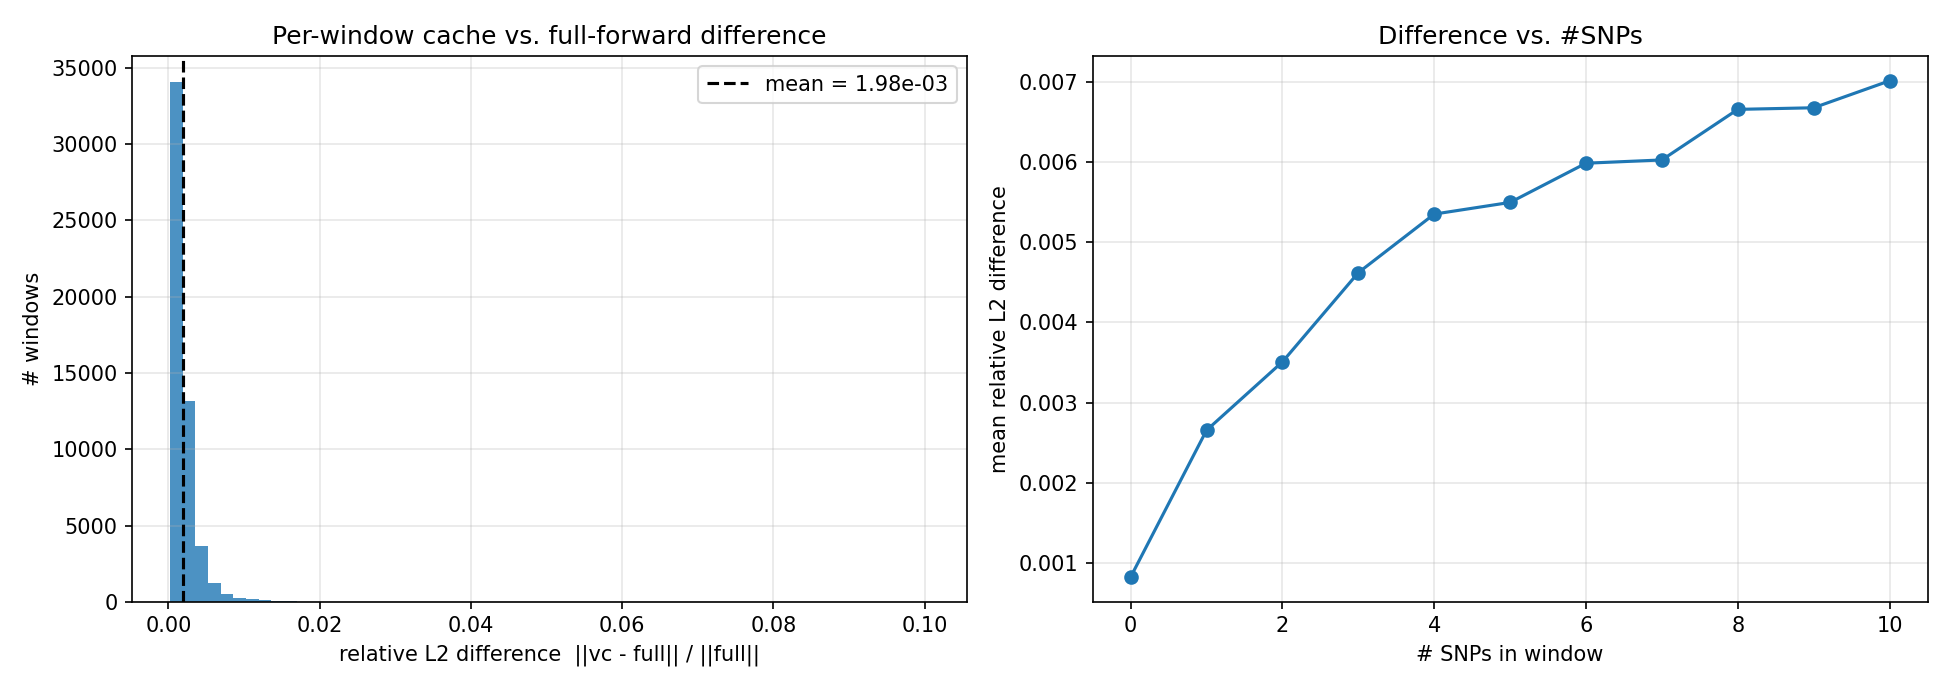
\includegraphics[width=0.7\linewidth]{13_vc_vs_fullforward.png}
  \caption{Per-window $L^2$ difference between variant-cache and full-forward
  window embeddings, relative to the embedding norm.}
  \label{fig:bitwise}
\end{figure}

\section{Discussion}
\label{sec:discussion}
The variant cache turns the redundancy of a near-reference cohort into a
\cacheFactor{} reduction in full language-model forwards while staying faithful
to the model it approximates: near-exact embeddings at the per-SNP-token level
(Section~\ref{sec:exp-fidelity}), unchanged downstream trait prediction and
population structure (Sections~\ref{sec:exp-head}--\ref{sec:exp-bitwise}), and
enough fidelity to fine-tune autoregressively on the SNP-prediction objective
(Section~\ref{sec:exp-ar}). The approximation is the frozen-reference assumption,
whose error grows only mildly with concurrent SNPs and is bounded by the window
design (Section~\ref{sec:exp-window}).

\bibliographystyle{plain}
\bibliography{refs}

\end{document}
